\documentclass{article}
% GENERAL
\usepackage{setspace,mathtools,amsfonts,amsmath,amsthm,amssymb,hyperref}
\usepackage{tikz,epigraph,pgfplots}  % For trees
\usepackage[utf8]{inputenc}
\usepackage{tikz-qtree,tikz-qtree-compat}
\usepackage{forest}

% FOR SOURCE CODE
\usepackage{listings}
% Default settings for code listings
\lstset{frame=tb,
  aboveskip=3mm,
  belowskip=3mm,
  showstringspaces=false,
  columns=flexible,
  basicstyle={\small\ttfamily},
  numbers=none,
  numberstyle=\tiny\color{gray},
  keywordstyle=\color{blue},
  commentstyle=\color{dkgreen},
  stringstyle=\color{mauve},
  frame=single,
  breaklines=true,
  breakatwhitespace=true
  tabsize=4
}

% FOR TREE DRAWING
\pgfplotsset{compat=newest}
\usetikzlibrary{shapes.geometric,arrows,fit,matrix,positioning}
\tikzset
{
      treenode/.style = {circle, draw=black, align=center, minimum size=1cm}
}

% MARGINS
\usepackage[left=1in,top=1in,right=1in,bottom=1in]{geometry}
\onehalfspacing

\begin{document}
\title{CMPT 419 Assignment 2}
\author{Colin Woodbury\\ 301238755\\ cwoodbur@sfu.ca}
\date{\today}
\maketitle

% --- TABLE OF CONTENTS ---
\tableofcontents
\clearpage
% -------------------------

\section{Linear Model for Classification}

\begin{center}
  \includegraphics[scale=0.75]{dbs}
\end{center}

A point is assigned to class $C_k$ if $y_k(\mathbf{x}) > y_j(\mathbf{x})$
for all $j \neq k$. Since we already know the decision boundaries and
points that lay on them, we need only to choose three planes of the
form $y_k(\mathbf{x}) = \mathbf{w}^T_k\mathbf{x} + w_k0$ that match the
above criteria.\\

The points $(-1,0,0)$ and $(0,-1,0)$ lie on the decision boundary of
Class 1 and 2. Since there are an infinite number of planes that intersect
this boundary, we choose an arbitrary third point to constrain the solution,
such that this plane will yield the highest height among the three, given
$\mathbf{x}$ values in the Class 1 area.
Let this point be $(-1,-1,1)$. Solving for the equation of a plane,
we find:

\begin{align*}
  y_1(\mathbf{x}) &= -1x_1 - 1x_2 - 1\\
  \text{Given: } \mathbf{w^T} &= (-1,-1)\\
  w_0 &= -1
\end{align*}

We solve for $y_3$ in a similar fashion. The two points on this plane
are $(1,0,0)$ and $(0,1,0)$. Let a third points be $(1,1,1)$. Solving
for the plane in the same way, we have:

\begin{align*}
  y_3(\mathbf{x}) &= 1x_1 + 1x_2 - 1\\
  \text{Given: } \mathbf{w^T} &= (1,1)\\
  w_0 &= -1
\end{align*}

$y_2$ is the simplest. Since both $y_1$ and $y_3$ have negative values
in $\mathbf{w}^T\mathbf{x} + w_0$ space within the Class 2 area,
the plane for Class 2 can sit parallel to the feature space. Specifically:

\begin{align*}
  y_2(\mathbf{x}) &= 0
\end{align*}

\section{Kernels}

\begin{enumerate}
\item How do the coefficients affect the model for:
  \begin{itemize}
  \item \textbf{unregularized regression?} \fbox{They wouldn't},
    as the weights would
    compensate and be lower to minimize the squared error.
  \item \textbf{regularized regression?} \fbox{They would}. If preceded
    by a coefficient like $\sqrt{2} > 1$, the weight for that
    term will be smaller to compensate (as above). Since it is less,
    the $\lambda$ won't affect it as strongly, resulting in a fitted curve
    that isn't as accurate as the true source curve.
  \end{itemize}

\item Combining Kernels. As is typical for proofs like these,
  we expand terms and simplify to show that this corresponds to a dot product.
  \begin{proof}
    \begin{align*}
      k_c(x,z) &= \alpha k_a(x,z) + \beta k_b(x,z)\\
      &= \alpha(\phi_1^a(x),\ldots,\phi_N^a(x))(\phi_1^a(z),\ldots,\phi_M^a(z))^T + \beta(\phi_1^b(x),\ldots,\phi_N^b(x))(\phi_1^b(z),\ldots,\phi_M^b(z))^T\\
      &= \alpha[\phi_1^a(x)^T\phi_1^a(z) + \cdots + \phi_N^a(x)^T\phi_N^a(z)] + \beta[\phi_1^b(x)^T\phi_1^b(z) + \cdots + \phi_M^b(x)^T\phi_M^b(z)]\\
      &= \alpha\phi_1^a(x)^T\phi_1^a(z) + \cdots + \alpha\phi_N^a(x)^T\phi_N^a(z) + \beta\phi_1^b(x)^T\phi_1^b(z) + \cdots + \beta\phi_M^b(x)^T\phi_M^b(z)\\
      &= (\alpha\phi_1^a(x),\ldots,\alpha\phi_N^a(x),\beta\phi_1^b(x),\ldots,\beta\phi_M^b(x))(\phi_1^a(z),\ldots,\phi_N^a(z),\phi_1^b(z),\ldots,\phi_M^b(z))^T\\
      &\text{which is clearly the dot product on mappings of the two input vectors}
    \end{align*}
  \end{proof}
\end{enumerate}

\section{Logistic Regression}

\begin{enumerate}
\item Plots
  \begin{center}
  \includegraphics[scale=0.75]{3-1b}
  \includegraphics[scale=0.75]{3-1c}
\end{center}

  To choose a good decision boundary, we are performing regression on a line.
  We minimize our error function (a bowl-like shape in error space) via
  Gradient Descent. The step size is a small enough value that it finds the
  bowl quickly without overshooting it, but then proceeds to bounce between
  the sides of the bowl as it iterates toward the minimum. This bouncing
  must mean the algorithm thinks it is taking a more efficient step
  by moving across the valley, instead of moving straight down.\\

  These zig-zag steps in the error yield near-mirrored $\mathbf{w}$ values,
  which gives us an oscillating decision boundary, and thus an
  oscillating intersept/slope curve.
  
\item Plot
  \begin{center}
    \includegraphics[scale=0.75]{3-2}
  \end{center}

  $\eta = 0.003$ remains the optimal value. A larger value seems to
  converge slower.\\
  Notice that the three smallest values don't cause the descent to oscillate.
  In this way, they can be thought to be ``better'' as they take a more
  direct path to the minimum.
  They also converge slower, but that is to be expected.

\item Stochastic Gradient Descent
  \begin{center}
    \includegraphics[scale=0.75]{3-3}
  \end{center}

  \emph{Note:} The sudden drop to 0 for three of the $\eta$ values
  represents convergence. No data was recorded after that point, so
  Matlab likely padded the vectors' remaining columns with 0's.\\
  
  Both this plot and the one from the question above appear to be
  converging on the same likelihood value. The two only share two equal
  step sizes, 0.001 and 0.0001. Comparing those, it appears SGD to be
  slower than normal gradient descent. However, with higher step sizes,
  SGD actually converges, where GD never did.

\item IRLS
  \begin{center}
  \includegraphics[scale=0.75]{3-4a}
  \includegraphics[scale=0.75]{3-4b}
\end{center}
\end{enumerate}

\section{Kernelized Perceptron}
This was an interesting problem that had me dedicate many hours to it.\\
I tested with two kernels, the supplied \textbf{Gaussian} kernel and a
\textbf{Hyperbolic Tangent} (Sigmoid) kernel, defined by:

\begin{align*}
  k(x,y) = \tanh(\alpha x^Ty + c)
\end{align*}

where I set $\alpha$ to be $\frac{1}{N}$, where $N$ is the size of the
data set (apparently this is typical). $c$ is the slope hyperparameter,
but no matter what I set it to, I had validation error rates consistantly
around 25 to 30 percent.\\

The Gaussian kernel, on the other hand, given $\sigma = 15$ instead
of the default 5 gave fairly good results:

\begin{center}
  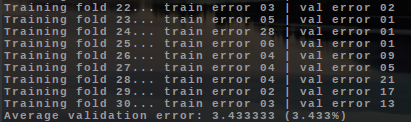
\includegraphics{gauss-15}
\end{center}

This is what I used to produce my final Fn for submission.

\end{document}
